\documentclass[10pt]{article}

\usepackage[margin=0.75in]{geometry}
\usepackage{amsmath,amsthm,amssymb}
\usepackage{xcolor}
\usepackage{cancel}
\usepackage{graphicx}
\usepackage{changepage}
\usepackage{circuitikz}
\usepackage{pgfplots}
\usepackage{physics}
\usepackage{hyperref}
\usepackage{siunitx}
\usepackage[breakable]{tcolorbox}
\usepackage[inline]{enumitem}

\theoremstyle{definition}
\newtheorem{problem}{Problem}
\newtheorem{soln}{Solution}

\pgfplotsset{compat=newest}
\usetikzlibrary{lindenmayersystems}
\usetikzlibrary{arrows}
\usetikzlibrary{calc}

\definecolor{incolor}{HTML}{303F9F}
\definecolor{outcolor}{HTML}{D84315}
\definecolor{cellborder}{HTML}{CFCFCF}
\definecolor{cellbackground}{HTML}{F7F7F7}
\newcommand{\eq}{=}
\usetikzlibrary{positioning, fit, calc}
\pgfdeclarelayer{background}  
\pgfsetlayers{background,main}
\DeclareSIUnit[number-unit-product = {\,}]\calorie{cal}
\DeclareSIUnit[number-unit-product = {\,}]\atmosphere{atm}
\AtBeginDocument{\RenewCommandCopy\qty\SI}

\makeatletter
\newcommand{\boxspacing}{\kern\kvtcb@left@rule\kern\kvtcb@boxsep}
\makeatother
\newcommand{\prompt}[4]{
    \ttfamily\llap{{\color{#2}[#3]:\hspace{3pt}#4}}\vspace{-\baselineskip}
}

\newcommand{\thevenin}[2]{
  \begin{center}
    \begin{circuitikz} \draw
      (0,0) -- (2,0) to[battery1, l_=$V_{Th}\eq#1$] (2,2) 
      to[resistor, l_=$R_{Th}\eq#2$] (0,2)
      ;
      \draw [o-] (-.07,2.079);
      \draw [o-] (-.07,0.079);
    \end{circuitikz}
  \end{center}
}

\newcommand{\norton}[2]{
  \begin{center}
    \begin{circuitikz} \draw
      (0,0) -- (3,0) to[american current source, l_=$I_{N}\eq#1$] (3,2) -- (0,2) (2,0)
      to[resistor, l=$R_{N}\eq#2$] (2,2)
      ;
      \draw [o-] (-.07,2.079);
      \draw [o-] (-.07,0.079);
    \end{circuitikz}
  \end{center}
}

\newcommand{\highlight}[1]{\colorbox{yellow}{$\displaystyle #1$}}

\newcommand{\ti}[1]{\widetilde{#1}}

\NewDocumentCommand{\evalat}{sO{\big}mm}{%
  \IfBooleanTF{#1}
   {\mleft. #3 \mright|_{#4}}
   {#3#2|_{#4}}%
}

\title{Physics 2700H: Assignment I}
\author{Jeremy Favro}
\date{\today}

\begin{document}
\maketitle

% PROBLEM 1
\begin{problem}
An ideal gas undergoes the following reversible cycle:

\begin{enumerate}[label=(\roman*)]
  \item an isobaric expansion from the state (P1,V1) to the state (P1,V2)
  \item an isochoric reduction in pressure to the state (P2,V2)
  \item an isobaric reduction in volume to the state (P2,V1)
  \item an isochoric increase in pressure back to the original state (P1,V1)
\end{enumerate}
\begin{enumerate}[label=(\alph*)]
  \item What work is done on the gas in this cycle?
  \item If $P_1 = 3.0\unit{\atmosphere}$, $P_2 = 1.0\unit{\atmosphere}$, $V_1 = 1.0\unit{\liter}$ and $V_2 = 2.0\unit{\liter}$, how much work is done on the gas in traversing the cycle 100 times?
\end{enumerate}
\end{problem}
\begin{soln}~
  \begin{enumerate}[label=(\alph*)]
    \item ~\\
          \begin{center}
            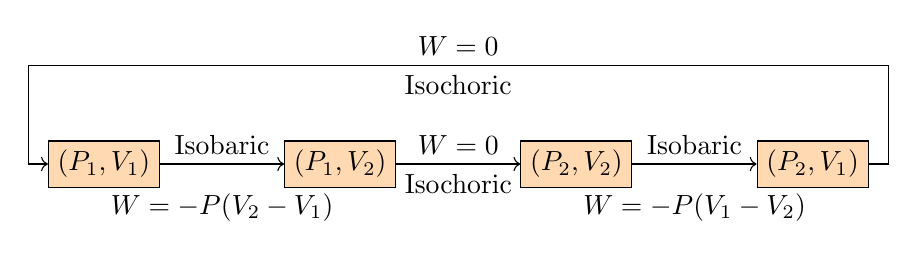
\begin{tikzpicture}
              \tikzstyle{block} = [rectangle, text centered, draw=black, fill=orange!30]
              \node (i) [block] {$(P_1,V_1)$};
              \node (ii) [block, right of=i, xshift=2cm]{$(P_1,V_2)$};
              \node (iii) [block, right of=ii, xshift=2cm]{$(P_2,V_2)$};
              \node (iv) [block, right of=iii, xshift=2cm]{$(P_2,V_1)$};
              \draw[->] (i) -- node[below, yshift=-0.25cm] {$W=-P(V_2-V_1)$} node[above] {Isobaric} (ii);
              \draw[->] (ii) -- node[above] {$W=0$} node[below] {Isochoric} (iii);
              \draw[->] (iii) -- node[below, yshift=-0.25cm] {$W=-P(V_1-V_2)$} node[above] {Isobaric} (iv);
              \draw[->] (iv.east) -| ++(0.25,1.25) -| node[xshift=5.46cm, above] {$W=0$} node[xshift=5.46cm, below] {Isochoric} ([xshift=-0.25cm]i.west) -- (i.west);
            \end{tikzpicture}
          \end{center}
          One cycle of work is therefore $-P_1(V_2-V_1)-P_2(V_1-V_2)$
    \item One hundred cycles of work is $100\left[\left(P_2-P_1\right)(V_2-V_1)\right]=\qty{-2.03d4}{\joule}$
  \end{enumerate}
\end{soln}

% PROBLEM 2
\begin{problem}
A hypothetical substance has an isothermal compressibility $\kappa = \frac{a}{v}$ and volume expansion coefficient $\beta=\frac{2bT}{v}$,
where $a$ and $b$ are constants and $v$ is the molar volume. Show that the equation of state is $$v-bT^2+aP=\mathrm{constant}$$
\end{problem}
\begin{soln}
  From equations 2.1 and 2.2 on the forumla sheet, $\displaystyle\beta=\frac{1}{V}\frac{\partial V}{\partial T}_P=\frac{2bT}{v}$ and
  $\displaystyle\kappa=-\frac{1}{V}\frac{\partial V}{\partial P}_T=\frac{a}{v}$ then,
  \begin{align*}
     & dV=\frac{\partial V}{\partial T}dT+\frac{\partial V}{\partial P}dP\rightsquigarrow\mathrm{ (chain\,rule)} \\
     & dV=\frac{2bVT}{v}dT-\frac{Va}{v}dP=2bnTdT-andP                                                            \\
     & V=bnT^2-anP+C                                                                                             \\
     & \frac{V}{n}=v=bT^2-aP+C                                                                                   \\
     & C=aP-bT^2+v=v-bT^2+aP                                                                                     \\
  \end{align*}
  Note that $C$ changes a bit here sign wise and gets divided by $n$ but it remains constant so I have left it as $C$.
\end{soln}

% PROBLEM 3
\begin{problem}
Researchers from the Universities of Maryland and Vermont found that adults' daily energy needs at rest (their resting metabolic rate, RMR)
is closely related to the mass of their bones \& muscles \& organs. By selecting any person from this data set, find:
\begin{enumerate}[label=(\alph*)]
  \item Their total bone/muscle/organs mass and their RMR in $\unit{\kilo\calorie\per\day}$.
  \item Their minimum daily energy needs written in $\unit{\joule}$, in $\unit{\kilo\joule}$, and in $\unit{\mega\joule}$.
  \item Their heat output at rest in watts (to high accuracy all energy we use at rest ends up emitted as heat).
\end{enumerate}
\end{problem}
\begin{soln}~
  \begin{enumerate}[label=(\alph*)]
    \item There are a few individuals at around $\qty{1500}{\kilo\calorie\per\day}$ and $60\unit{\kilo\gram}$ so I will work with an ideal individual
          at exactly these values.
    \item $\qty{1500}{\kilo\calorie\per\day}=6276000\unit{\joule}=6276\unit{\kilo\joule}=6.276\unit{\mega\joule}$
    \item $\displaystyle\frac{6276000\unit{\joule}}{86400\unit{\second}}=72.64\unit{\watt}$
  \end{enumerate}
\end{soln}

% PROBLEM 4
\begin{problem}
A gas is contained in a cylinder fitted with a frictionless piston and is taken from state a to state b along the path acb shown in Figure 3.8.
$80\unit{\joule}$ of heat flows into the system, and the system does $30\unit{\joule}$ of work.
\begin{enumerate}[label=(\alph*)]
  \item If instead the work done by the gas system is only $10\unit{\joule}$ along adb, how much heat flows into the system?
  \item When the system is returned from b to a along the curved path, the work done on the system is $20\unit{\joule}$. What is the heat transfer?
  \item If $U_a = 0$ and $U_d = 40\unit{\joule}$, find the heat absorbed in the processes ad and db.
\end{enumerate}
\end{problem}
\begin{soln}~
  \begin{enumerate}[label=(\alph*)]
    \item Net system energy change must be conserved so if work \textbf{done by the system} decreases by $20\unit{\joule}$ heat \textbf{into the system} must decrease by $20\unit{\joule}$ meaning that the new heat flow must be $60\unit{\joule}$
    \item We've kept the change in energy of the system as $50\unit{\joule}$ by the first law of thermodynamics for the first two processes. Because work is path-independent, the change in energy along
          the curved path is the same as the change in energy along acb but with reversed sign as we are going backwards. So, $\Delta U=-50\unit{\joule}=Q+20\unit{\joule}\implies Q=-70\unit{\joule}$.
    \item For ad, $\Delta U =40\unit{\joule}$, then for db we know that the total change must be $50\unit{\joule}$ in process ab, so $50\unit{\joule}=40\unit{\joule}+\Delta U_{db}\implies \Delta U_{db}=10\unit{\joule}$
  \end{enumerate}
\end{soln}

% PROBLEM 5
\begin{problem}
You have a pure metal that is unknown except for the fact that it happens to be among those listed in Table 3.1. A $36.7\unit{\gram}$ piece of this metal
at $50.0\unit{\celsius}$ is placed in a calorimeter containing $150\unit{\gram}$ of water, initially at $10\unit{\celsius}$. The final equilibrium temperature in the calorimeter is $12.0\unit{\celsius}$.
What is the metal?
\end{problem}
\begin{soln}
  Heat is the same between the water and the metal at equilibrium because they are in (presumably) perfect thermal contact so, with subscript m denoting metal and w denoting water,
  \begin{align*}
     & m_mc_m\Delta T_m=m_wc_w\Delta T_w                                  \\
     & c_m=\frac{m_wc_w\Delta T_w}{m_m\Delta T_m}\approx-900\unit{\joule} \\
  \end{align*}
  So, according to the table this metal is likely aluminum. I am not sure about the sign but it is kind of irrelevant I think, mostly because logically if it takes $-900\unit{\joule}$ ($\unit{\joule\per{\kilogram\celsius}}$, really) to cool
  something it will logically take $900\unit{\joule}$ to heat it up.
\end{soln}

% PROBLEM 6
\begin{problem}
A gas with adiabatic exponent $\gamma$ is compressed adiabatically from an initial state $(P_i, V_i)$ to final state $(P_f, V_f)$.
\begin{enumerate}[label=(\alph*)]
  \item Show that the work done in this process is $W=\displaystyle\frac{P_iV_i}{\gamma-1}\left[\left(\frac{V_i}{V_f}\right)^{\gamma-1}-1\right]$
  \item Evaluate the result numerically for one mole of helium gas initially at $P=1.0\unit{\atmosphere}$ and $T=300\unit{\kelvin}$ compressed to half its initial volume.
  \item Compute the work done in an isothermal compression from the same initial point to half the initial volume.
        Explain the difference between the numerical results for work done in adiabatic and isothermal compression.
\end{enumerate}
\end{problem}
\begin{soln}~
  \begin{enumerate}[label=(\alph*)]
    \item Starting with $dW=-PdV$ we can recognize that because this process is adiabatic $\displaystyle P=\frac{P_iV_i^\gamma}{V^\gamma}\left(=\frac{P_fV_f^\gamma}{V^\gamma}\right)$
          \begin{align*}
             & dW=-PdV                                                                                                                    \\
             & W=-\int_{V_i}^{V_f}\frac{P_iV_i^\gamma}{V^\gamma}\,dV\rightsquigarrow V_n^\gamma \text{ is constant}                       \\
             & W=-P_iV_i^\gamma\int_{V_i}^{V_f}V^{-\gamma}\,dV                                                                            \\
             & W=-\frac{P_iV_i^\gamma}{1-\gamma} \eval{V^{1-\gamma}}_{V_i}^{V_f} \rightsquigarrow \text{ assume } \gamma\neq1             \\
             & W=-\frac{P_iV_i^\gamma}{1-\gamma} \left[V_f^{1-\gamma}-V_i^{1-\gamma}\right]                                               \\
             & W=\frac{P_iV_i^{\cancel{\gamma}} V_i^{1-\cancel{\gamma}}}{\gamma-1} \left[\left(\frac{V_f}{V_i}\right)^{1-\gamma}-1\right] \\
             & W=\frac{P_iV_i}{\gamma-1} \left[\left(\frac{V_i}{V_f}\right)^{\gamma-1}-1\right]                                           \\
          \end{align*}
    \item $\gamma=1.66$ for approximately room temperature Helium\footnote{White, Frank M. (1998). Appendix A. Fluid Mechanics (4th ed.) (pp. 769-773). McGraw Hill.}
          \begin{align*}
             & V=\frac{nRT}{P}\implies W=\frac{nRT}{\gamma-1} \left[2^{\gamma-1}-1\right]=2192\unit{\joule} \\
          \end{align*}
    \item $dW=-PdV$ and $\displaystyle P=\frac{nRT}{V}=\frac{RT}{V}$ so
          \begin{align*}
             & W=-RT\int_{V_i}^{V_f}\frac{1}{V}dV                                                                      \\
             & =-RT\left[\ln V_f - \ln V_i\right]                                                                      \\
             & =-RT\ln\left(\frac{V_f}{V_i}\right)=-RT\ln\left(\frac{V_i}{2V_i}\right)=RT\ln 2\approx1729\unit{\joule}
          \end{align*}
          Because $\Delta U$ is the same for an adiabat as it is for an isotherm, $\Delta U = Q+W$ holds for both. In the case of an adiabat, $Q=0$ by definition so $W$ increases 
          (compared to an isotherm between the same two states) to ``take up the slack''. 
  \end{enumerate}
\end{soln}
\end{document}